% ********** Chapter 4 **********
\chapter{Solution}
\label{sec:Solution}

There are two kind of connection solution of the core of Web Call, the Relay Call and Third Party Call. The different between them is the way they handle media stream.

The Relay Call Controller works as a back-to-back agent and forwards media streams, while Third Party Call Controller only establishes connections by sending out SIP messages and it does not handles any streams itself. 

\section{Relay Call}
\label{sec:Solution:RelayCall}

\begin{figure}[!hbtp]
\centering
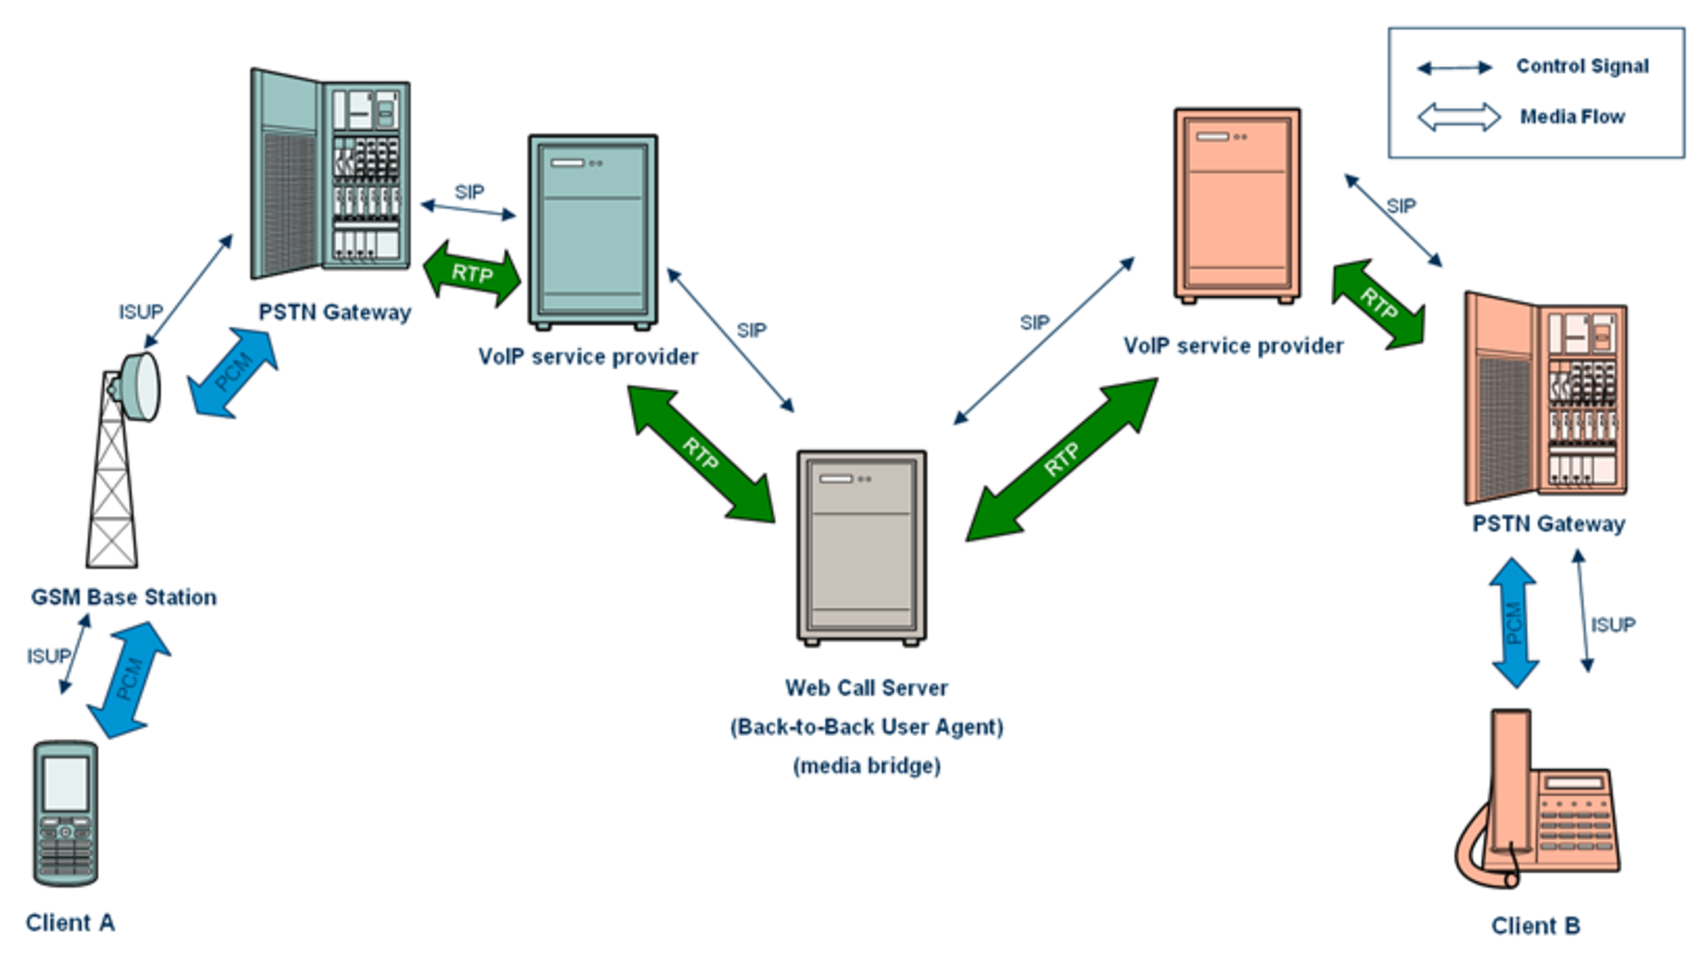
\epsfig{file=chap04/resources/the_signal_and_media_flow_of_relay_call, width=5.34in}
\caption{The signal and media flow of Relay Call}
\label{fig:TheSignalAndMediaFlowOfRelayCall}
\end{figure}

The signal and media flow of Relay Call is shown in Figure \ref{fig:TheSignalAndMediaFlowOfRelayCall}. In this scenario, the Web Call Example Application acts as a back-to-back user agent. It sets up the connection and forwards the media stream. It can be seen from the picture that both signal and media are handled by Web Call Server. When it starts, it try to call client A. After it establishes a session with client A, it will try to call client B and also establish a session with client B. After that, it will work as a media stream bridge and forward media stream from client A to B, as well as from client B to A.

For a detail description and mechanism of Relay Call, please refer to the master thesis of \textbf{Web Call SDK} by \textit{Yuening Chen}\cite{WebCallSDK}.

\section{Problem of Relay Call}
\label{sec:Solution:ProblemOfRelayCall}

\subsection{The Load on Controller}
\label{sec:Solution:ProblemOfRelayCall:TheLoadOnController}
 
The controller here acts as a back to back user agent (B2BUA). It receives the RTP flow from one client and transfers it to another client. It does the same in the opposite direction. That means all of the RTP traffic will go through the controller. So the load on controller will be heavier as with the number of concurrent users increases. A powerful host is needed to handle the RTP flows. However the design goal of Web Call SDK was simply a tool kit that can easily be integrated into a web site. Unfortunately, this  current mechanism of session control will decrease the performance of whole web site. 

\subsection{The Latency of Audio}
\label{sec:Solution:ProblemOfRelayCall:TheLatencyOfThePhoneCall}
 
As can be seen from the session flow, the RTP goes from one client to the controller via a SIP provider and then the controller transfers the RTP to another client via the SIP provider again. This means that each direction of RTP will go through SIP provider twice. So the latency of the phone call via the SIP provider will be double that of normal calls.  The latency of phone-to-phone call via Web Call SDK test turned to be more then 2 seconds. It is quite unacceptable. 

\subsection{Lack of Reliability}
\label{sec:Solution:ProblemOfRelayCall:LackOfReliability}

Since all of RTP flows go through the controller, thus if the controller crashes, all of calls will be immediately interrupted. 

\section{Third Party Call}
\label{sec:Solution:ThirdPartyCall}

In the traditional telephony context, third party call control allows one entity (which we call the controller) to set up and manage a communications relationship between two or more other parties. Third Party call control (referred as 3pcc) is often used for operator services (where an operator creates a call that connects two participants together) and for conferencing. The signal and media flow in third party call is show in Figure \ref{fig:TheSignalAndMediaFlowOf3pc} The advantage of third party call in Web Call is that the controller only need to handle message transfer and leaves the media flow for the ISP.

\begin{figure}[!hbtp]
\centering
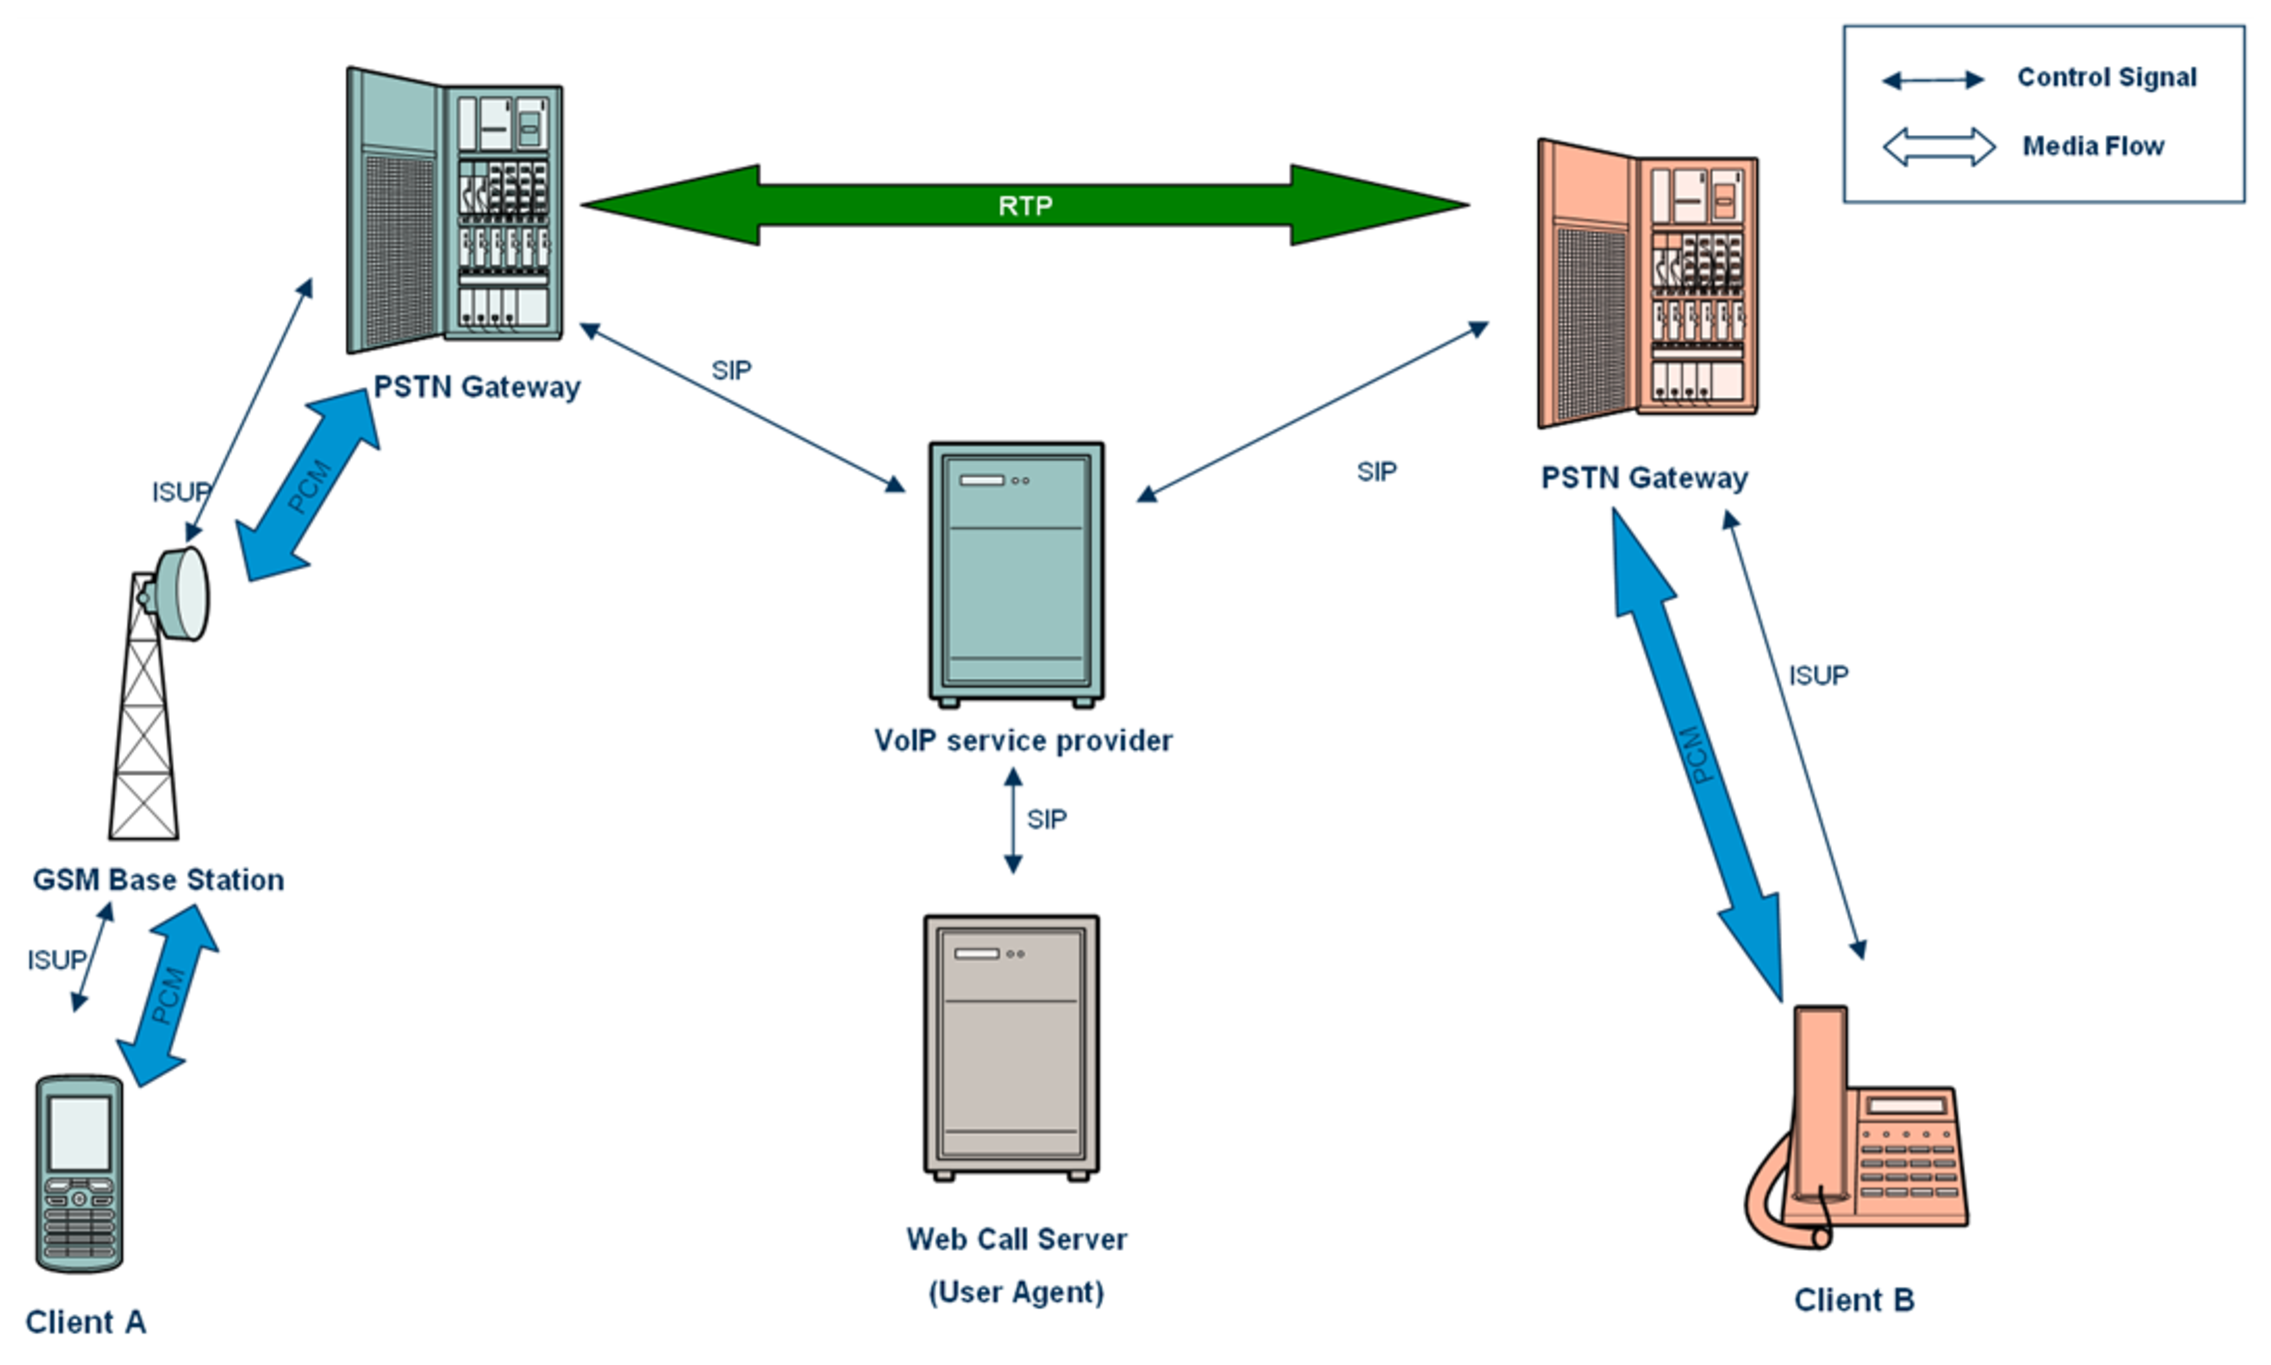
\epsfig{file=chap04/resources/the_signal_and_media_flow_of_3pc, width=5.34in}
\caption{The signal and media flow of Third Party Call}
\label{fig:TheSignalAndMediaFlowOf3pc}
\end{figure}

\subsection{Call Transfer}
\label{sec:Solution:ThirdPartyCall:CallTransfer}

The call transfer implementation use a \texttt{REFER} method which defined in \textit{The Session Initiation Protocol (SIP) Refer Method} (RFC \nobreak \nobreak{3515})\cite{RFC3515}. ``The \texttt{REFER} method indicates that the recipient (identified by the Request-URI) should contact a third party using the contact information provided in the request''\cite{RFC3515}. 

The Call flow is shown in Figure \ref{fig:CallTransfer}. The controller first sends an \texttt{INVITE} to client A (1). This invite is just a normal invite. A's phone rings and answers. This results in a \texttt{200 OK} (2). The controller then answer client A an \texttt{ACK} (3). Follow that, the controller send out a \texttt{REFER refer-to}: Client B (4), which means controller wish client A to make a phone call to client B. The client A understands that and returns a \texttt{200 \nolinebreak OK} to controller (5). Then client A sends an \texttt{INVITE referred-By}: C to client B (6). Client A and Client B can establish a session according the \texttt{INVITE} from A to B.  The \texttt{BYE} (8) and \texttt{200 \nolinebreak OK} (9) means the controller cut the media stream between itself and client A. 

To accomplish the whole call flow, client A must support RFC3515.

\begin{figure}[!hbtp]
\centering
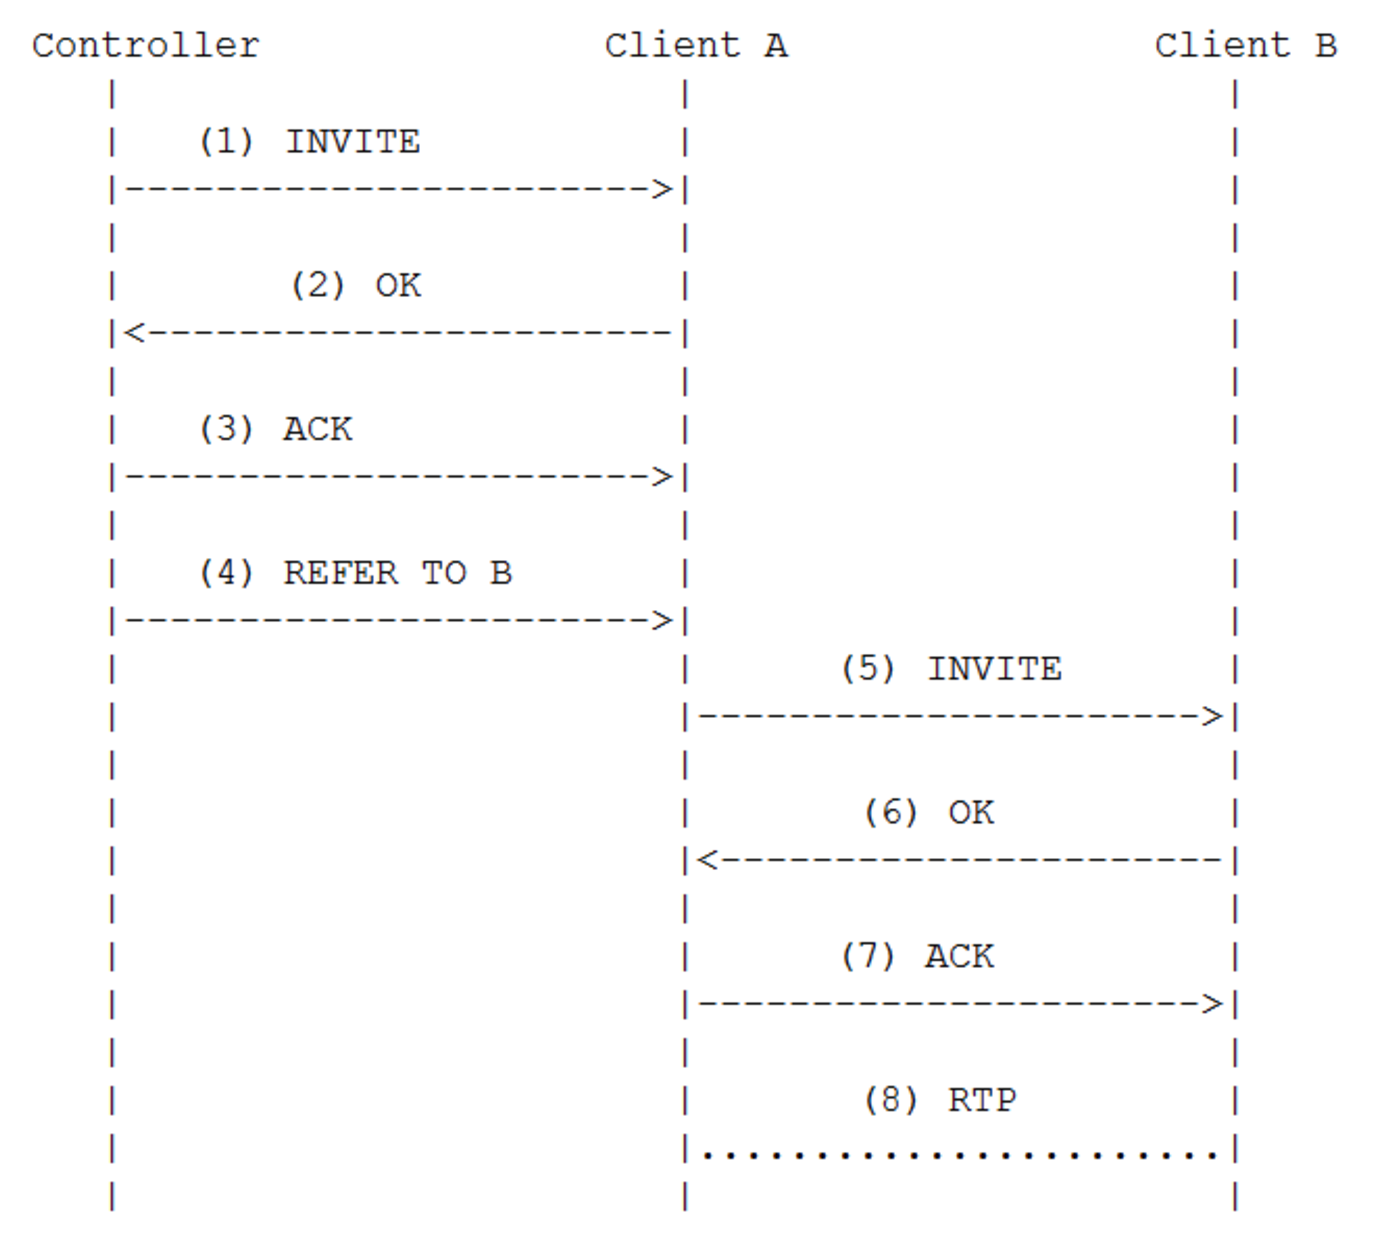
\epsfig{file=chap04/resources/call_transfer, width=5.34in}
\caption{The signal and media flow of Call Transfer}
\label{fig:CallTransfer}
\end{figure}

\subsection{SDP Swap}
\label{sec:Solution:ThirdPartyCall:SDPSwep}

This implementation of third party call control swaps SDP from two clients. The prototype of SDP swap comes from  \textit{Best Current Practices for Third Party Call Control (3pcc) in the Session Initiation Protocol (SIP)} (RFC \nolinebreak \nobreak{3725}). However, the call flow in RFC \nolinebreak \nobreak{3725} is quite complicated. The concept of \textbf{SDP Swep} is that controller calls to client and swaps two SDP which got from clients. These two clients seem to call controller but the media stream is connected directly between them.

The call flow of SDP swap implementation of third party call control is shown in Figure \ref{fig:SdpSwap}. Controller first call client A. This \texttt{INVITE} has no session description. Client A's phone rings, and client A answers. It results a \texttt{200 OK} (3) that contains an offer which contains client A's SDP \cite{RFC3261}. Meanwhile, the controller does the same to client B (2) and gets client B's offer (4) which contains client B's SDP. So far, controller has both client A and client B's SDP. It just simply swaps these two SDPs, then \texttt{ACK} client B with client A's SDP (5) and \texttt{ACK} client A with client B's SDP (6). So client A gets client B's SDP by (6) and client B gets client A's SDP by (5). Therefore, media flows between client A and client B (7).

\begin{figure}[!hbtp]
\centering
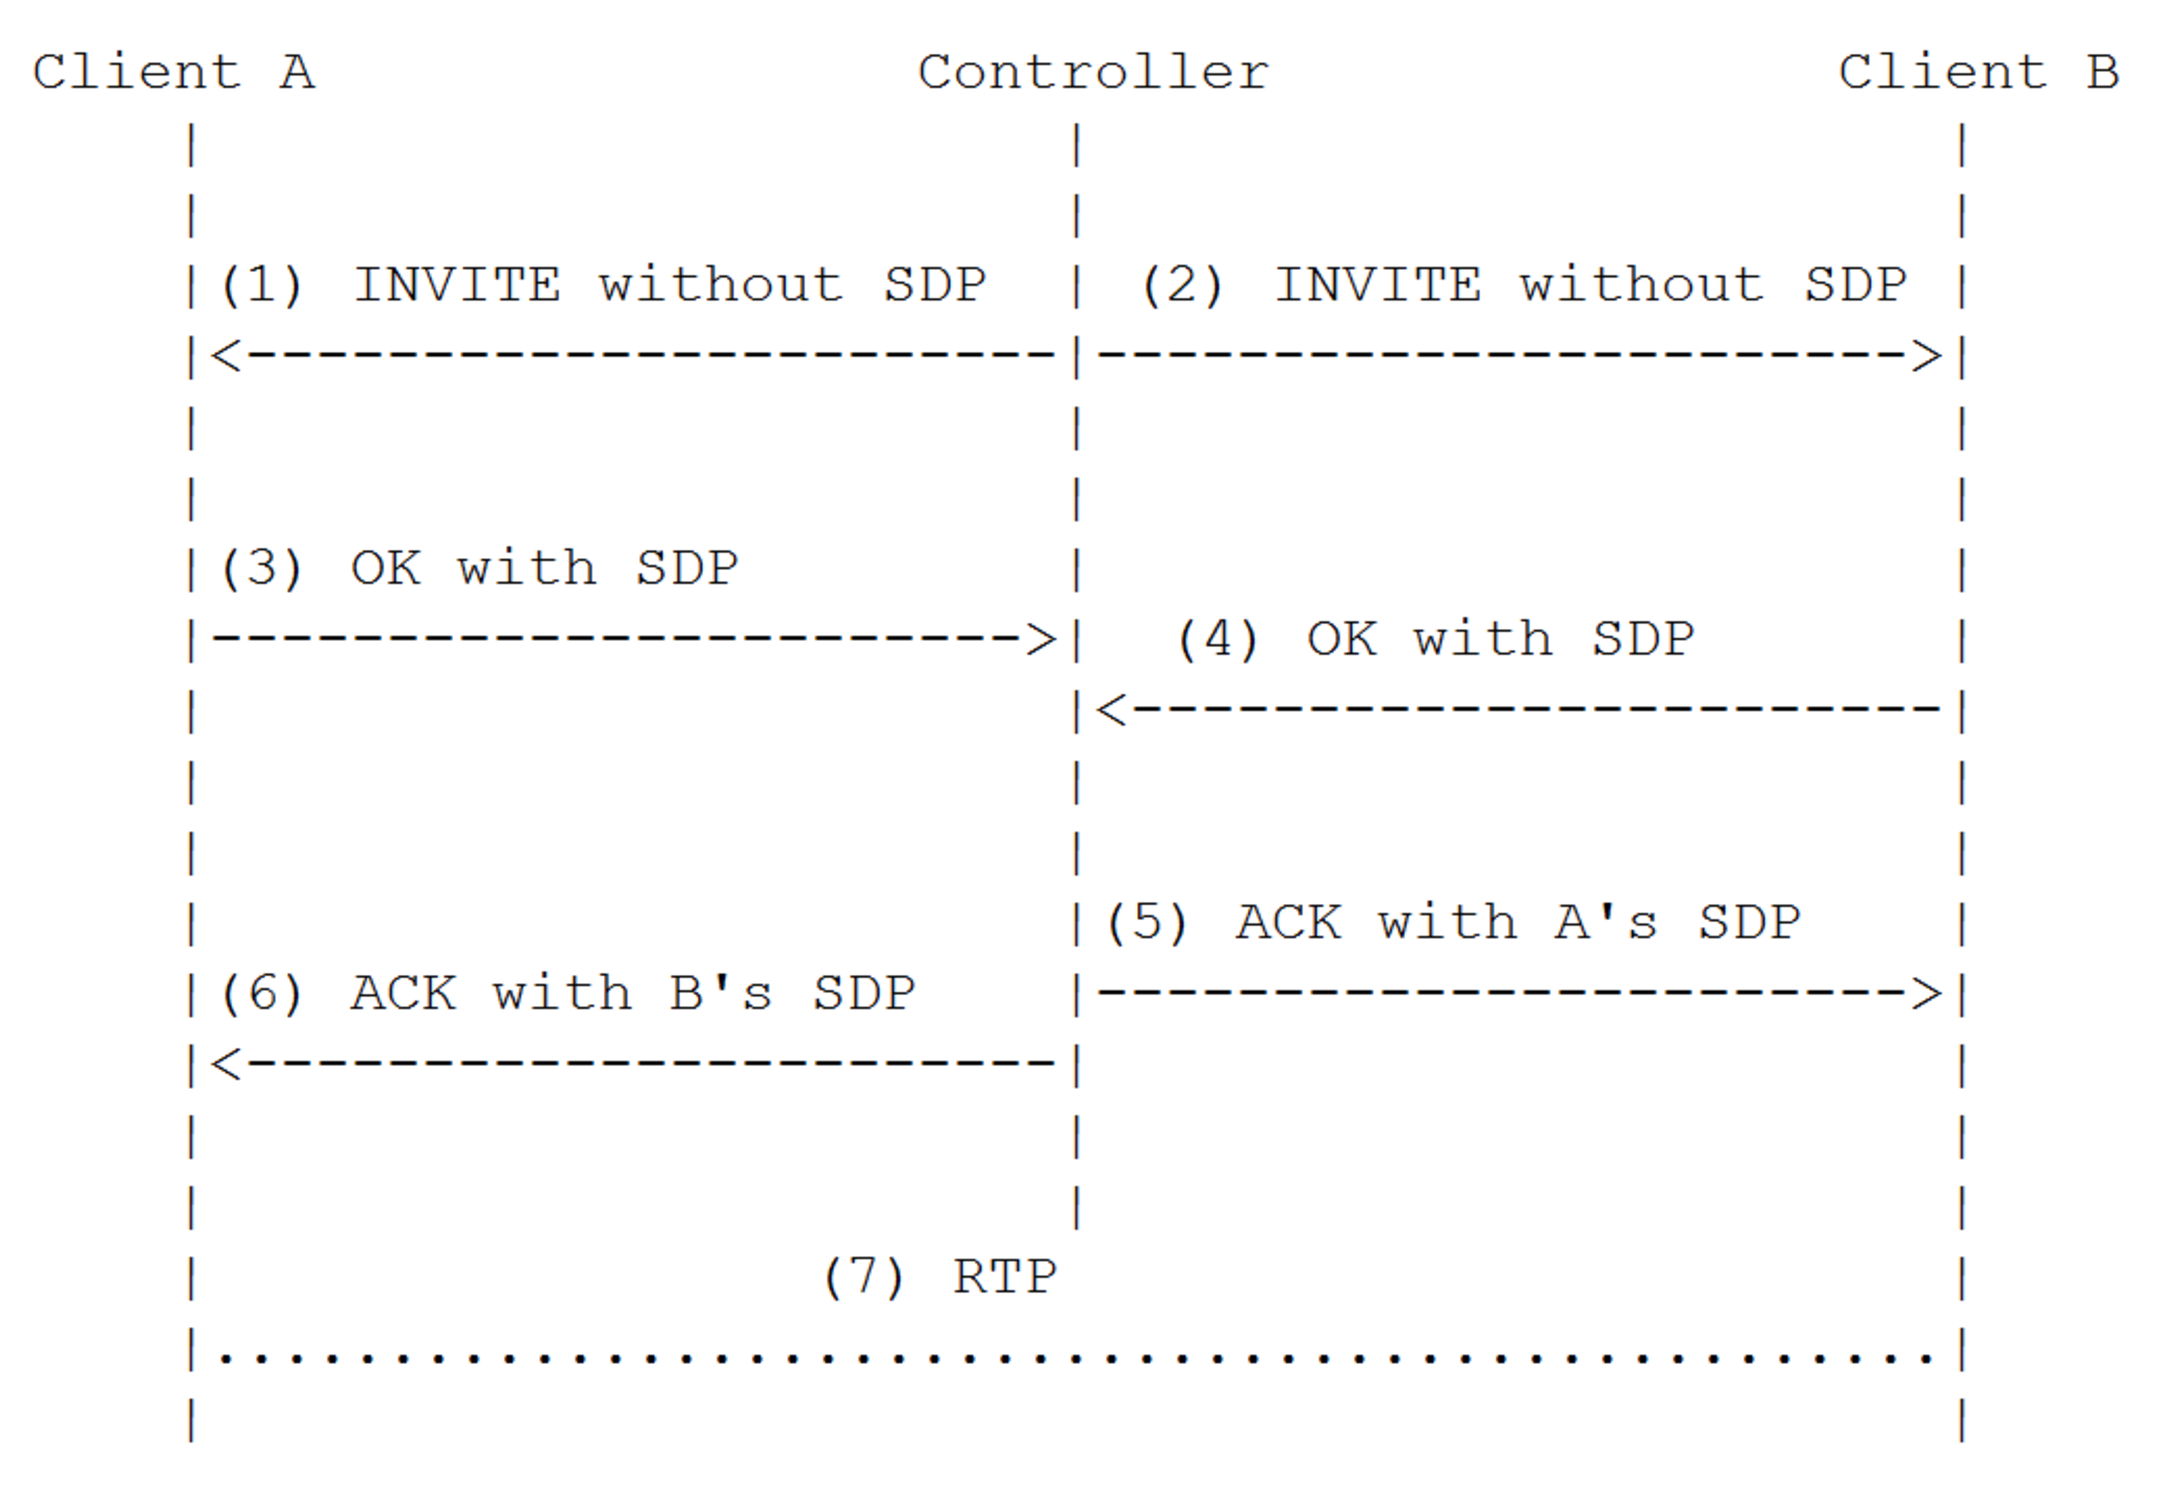
\epsfig{file=chap04/resources/sdp_swap, width=5.34in}
\caption{The signal and media flow of SDP Swap}
\label{fig:SdpSwap}
\end{figure}

\subsection{Re-invite}
\label{sec:Solution:ThirdPartyCall:Re-invite}

A \texttt{Re-INVITE} is used to change the session parameters of an existing or pending call. It uses the same Call-ID, but the CSeq is incremented because it is a new request. The Re-invite implementation send two client's SDP to each other in the Re-invite process. 

The call flow is shown in Figure \ref{fig:Re-invite}. From the SIP message (1) to (6), the controller uses a three way handshake to establish connections with client A and client B. In (3) and (4) the controller gets client A and client B's SDP which are going to be used in the Re-invite phase in (7) and (8). The controller sends a \texttt{Re-INVITE} to A with B's SDP (7), which indicates the controller changes its media port to B's. At the moment, controller also send a \texttt{Re-INVITE} to client B with client A's SDP, which indicates the controller change its media port to A's. Both client A and client B gets each other's SDP, thus, a media stream could be established between A and B (13).

\begin{figure}[!hbtp]
\centering
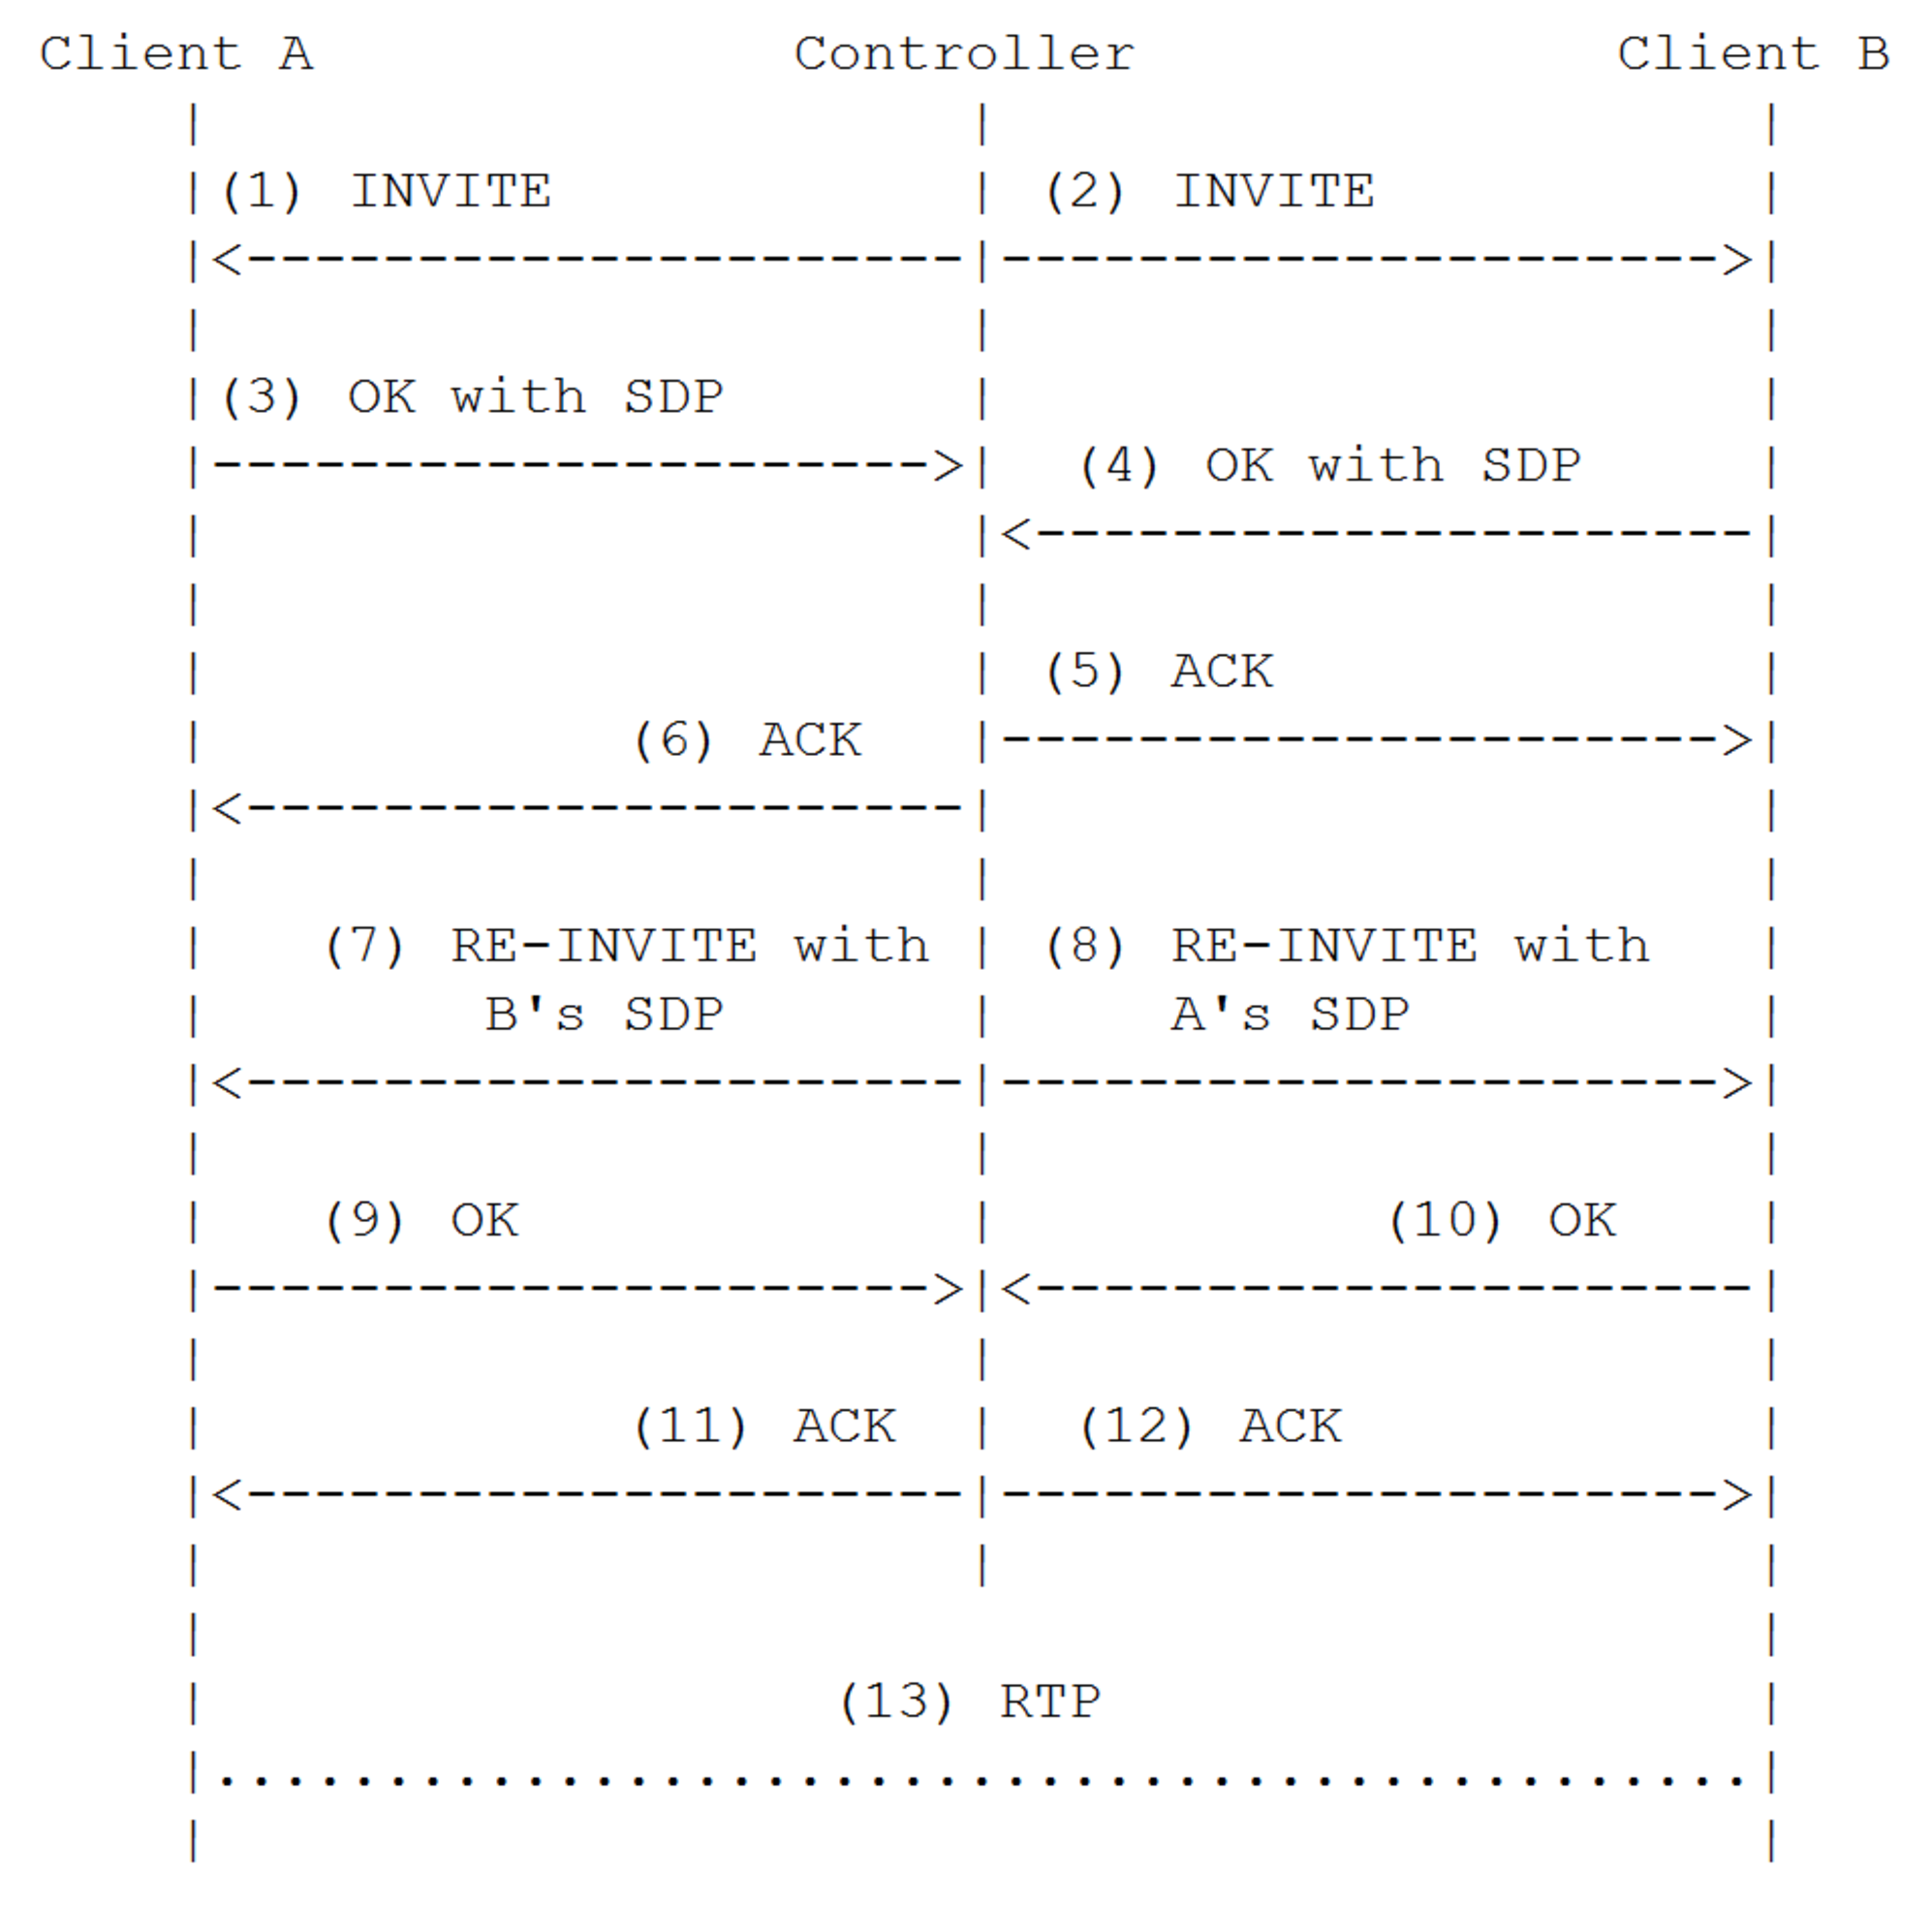
\epsfig{file=chap04/resources/re-invite, width=5.34in}
\caption{The signal and media flow of SDP Swap}
\label{fig:Re-invite}
\end{figure}

\subsection{Web Client}
\label{sec:Solution:ThirdPartyCall:WebClient}



\section{Conclusion}
\label{sec:Solution:Conclusion}

\begin{tabular}{|p{0.60in}|p{0.60in}|p{0.65in}|p{0.65in}|p{0.65in}|p{0.65in}|p{0.65in}|}
\hline
        & \multirow{3}{0.65in}{\textbf{PSTN}} &\multicolumn{5}{c|}{VoIP} \\ \cline{3-7}
        &               & \multirow{3}{0.65in}{\textbf{Relay Call}} &\multicolumn{4}{c|}{Third Party Call} \\ \cline{4-7}
 		  &               &                    & \textbf{Call Transfer} &\textbf{SDP Swap} &\textbf{Re-Invite} &\textbf{Web Client} \\\cline{1-7}	
\textbf{service provider} & All PSTN switch & \multirow{2}{0.65in}{support by all VoIP service providers} & \multicolumn{4}{c|}{Not support by all VoIP service providers}\\ \cline{4-7}
& & & The ones who support REFER method & The ones who do not filter SIP message which doesn't carry SDP & The ones who support
Re-Invite message & The ones who supply web site call \\ \cline{1-7}

\textbf{Client} & \multirow{2}{0.65in}{Traditional telephone or mobile phone} &\multirow{2}{0.65in}{All clients (traditional phone, mobile phone, software-client)} & \multicolumn{3}{p{1.95in}|}{Traditional phone, mobile phone, software-client, under particular requirements of software-client or PSTN gateway} & \multirow{2}{0.65in}{All clients (traditional phone, mobile phone, software-client)} \\ \cline{4-6}
& & & Client need support REFER method  & Client need implement RFC 3725 & Client need support Re-Invite & \\ \cline{1-7}
\textbf{Media Stream} & In PSTN network & Internet and/or PSTN, need to be handled on controller & \multicolumn{4}{c|}{Internet and/or PSTN}\\ \cline{1-7}
\textbf{Latency} & Very Short / QoS guarantee & long & \multicolumn{4}{c|}{Short, acceptable. But no QoS guarantee} \\ \cline{1-7}
\textbf{Cost} & Expensive (especially for international call ) & \multicolumn{5}{c|}{cheap} \\

\hline
\end{tabular}

% ********** End of chapter **********
